%!TEX program = xelatex
\documentclass[aspectratio=169]{ctexbeamer}
\usepackage{subfigure}
\usepackage{caption}
% \usepackage{physics}
% \usepackage{physics}  
                        %%% 宽高比说明 %%%%
%% ctexbeamer宏包支持各种宽高比,但本模板只适配了4:3(默认)和16:9的宽高比背景。
%% 添加选项aspectratio=169或aspectratio=43可以更改宽高比,默认是4:3
\usepackage[bluetheme]{ustcbeamer}
\input{ustctheme.tex}
                        %%% ustcbeamer说明 %%%%
%% 宏包使用了TikZ代码形式的背景文件(在子文件夹theme中),默认选项"bluetheme",是科大校徽的蓝色;此外ustcbeamer还内置了红色和黑色主题"redtheme","blacktheme"。

                        %%% 自定义你的主题颜色 %%%
%% 一旦使用了下述命令就会覆盖ustcbeamer的内置颜色选项,你可以设置自己喜欢的RGB色值:
% \definecolor{themecolor}{RGB}{0,150,0} % 这是绿色主题
% \definecolor{themecolor}{RGB}{0,150,150} % 青色主题,也蛮好看的

%% 注意小写rgb和大写RGB表示的色值相差255倍,即RGB{255,255,255}=rgb{1,1,1};
% \definecolor{themecolor}{rgb}{0,0.5,0.3} % 深绿色主题

%% 建议自定义的主题颜色选择偏深色
%%%%%%%%%%%%%%%%%%%%%%%%%%%%%%%%%%%%%%%%%%%%%%%%%%%%%%%%%%%%%%%%%%%%%%


\title[底部简明标题]{
    Jan 20 report
}
\author[底部演讲者]{报告人:王政}
\institute[USTC]{
中国科学技术大学,近代物理系
}
\date{\today}
\begin{document}
%\section<⟨mode specification⟩>[⟨short section name⟩]{⟨section name⟩}
%小于等于六个标题为恰当的标题

%--------------------
%标题页
%--------------------
\maketitleframe
%--------------------
%目录页
%--------------------
%beamer 101
%--------------------
%节目录页
%--------------------
\AtBeginSection[]{
\setbeamertemplate{footline}[footlineoff]%取消页脚
  \begin{frame}%
    \frametitle{Contents}
	%\tableofcontents[currentsection,subsectionstyle=show/hide/hide]%高亮当前节,不显示子节
    \tableofcontents[currentsection,subsectionstyle=show/show/hide]%show,shaded,hide
  \end{frame}
\setbeamertemplate{footline}[footlineon]%添加页脚
}
%--------------------
%子节目录页
%--------------------
\AtBeginSubsection[]{
\setbeamertemplate{footline}[footlineoff]%取消页脚
  \begin{frame}%
    \frametitle{Contents}
	%\tableofcontents[currentsection,subsectionstyle=show/hide/hide]%高亮当前节,不显示子节
    \tableofcontents[currentsection,subsectionstyle=show/shaded/hide]%show,shaded,hide
  \end{frame}
\setbeamertemplate{footline}[footlineon]%添加页脚
}


\section{Motivation}


\begin{frame}
  \frametitle{Motivation}
  \begin{columns}
    \begin{column}{0.5\textwidth}
      Motivation:
      \begin{itemize}
        \item measure the cross section of $e^+ e^- \to \phi K^+ K^-$ via ISR
        \item study the structure near 2.2324GeV which BaBar and BESIII have observed
        \item study the spectrum of M($K^+ K^-$)
      \end{itemize}
      Reference to:
      \begin{itemize}
        \item B.Aubert et al.(BaBar Collaboration),PhysRevD.86.012008(2012) 
        \item M.Ablikim et al.(BESIII Collaboration),PhysRevD.100.032009(2019)
      \end{itemize}

    \end{column}

    \begin{column}{0.5\textwidth}
       \includegraphics[width=0.8\textwidth]{figures/phikk.png}
      \includegraphics[width=0.8\textwidth]{figures/kkkk_nogreen.png}
    \end{column}
  \end{columns}
\end{frame}

\section{Data Sets}

\begin{frame}
  \frametitle{Data Sets}
	\begin{itemize}
    \item[$\star$] Data
    \begin{itemize}
    \item $\Upsilon(4S)$ : $360.531 fb^{-1}$
	  \item $\Upsilon(4S)$ off resonance :  $41.424 fb^{-1}$
	  \item $\Upsilon(5S)$ :  $19.34fb^{-1}$
    \item $\mathcal{L}_{tot} = 421.295\ \mathrm{fb}^{-1}$ (BaBar: $454\ \mathrm{fb}^{-1}$)
    \end{itemize}
    \item[$\star$] generic MC (MC15rd ,$\mathcal{L}_{gMC} = 4\mathcal{L}_{data}$)
    \begin{itemize}
      \item \texttt{/belle/collection/MC/MC15rd\_exp20-26\_4S\_v2}
      \item \texttt{/belle/collection/MC/MC15rd\_exp7-18\_4S\_v3}
    \end{itemize}
    \item[$\star$] SignalMC
    \begin{itemize}
      \item 10M run independent events generated by \texttt{PHOKHARA\_EvtGen}
    \end{itemize}
        \end{itemize}
\end{frame}

\section{Event Selection}

\begin{frame}
  \frametitle{Selection Criteria}
  \begin{columns}
    \begin{column}{0.5\textwidth}
      \begin{itemize}
        \item[$\star$] Charged track selection:
          \begin{itemize}
            \item $dr < 0.5$, $|dz| < 2$
            \item $N_{good} = 4$, $\sum Q = 0$
          \end{itemize}
        
        \item[$\star$] Photon selection:
          \begin{itemize}
            \item Select photon with highest energy
            \item $E \geq 3$ GeV
          \end{itemize}
          
        \item[$\star$] PID selection:
          \begin{itemize}
            \item $binaryPID = \frac{\mathcal{L}_{K}}{\mathcal{L}_k + \mathcal{L}_{\pi}} > 0.6$
            \item Number of good kaon $ \geq 3$
          \end{itemize}
          
        \item[$\star$] 3C kinematic fit:
          \begin{itemize}
            \item Event survives 3C fit
            \item $\chi^2 < 40$
          \end{itemize}
          
        \item[$\star$] $\phi$ mass window:
          \begin{itemize}
            \item $1.00133653 < M_{K^+K^-} < 1.03766347$
          \end{itemize}
          
        \item[$\star$] Select combination with minimum $\chi^2$
      \end{itemize}
    \end{column}
    \begin{column}{0.5\textwidth}
      \centering
      \includegraphics[width=0.75\textwidth]{figures/chisq_cut.png}
      
      \includegraphics[width=0.75\textwidth]{figures/sMC_phi_fit_0.png}
    \end{column}
  \end{columns}
\end{frame}




\begin{frame}
  \frametitle{insert Line Shape}
  \begin{columns}[t]
    \begin{column}{1.5\textheight}
      \begin{columns}
        \begin{column}{0.3\textwidth}
          \centering
          \includegraphics[width=\textwidth]{figures/phikk.png}
          \captionof{figure}{cross section}
        \end{column}
        \begin{column}{0.05\textwidth}
          \centering
          $\times$
        \end{column}
        \begin{column}{0.3\textwidth}
          \centering
          \includegraphics[width=\textwidth]{figures/eff_lumino.png}
          \captionof{figure}{effective luminosity}
        \end{column}
        \begin{column}{0.05\textwidth}
          \centering
          $=$
        \end{column}
        \begin{column}{0.3\textwidth}
          \centering
          \includegraphics[width=\textwidth]{figures/Nes.png}
          \captionof{figure}{estimate entries}
        \end{column}
      \end{columns}
    \end{column}
  \end{columns}

  \vspace{0.5cm}

  \begin{columns}[t]
    \begin{column}{1.3\textheight}
      \begin{columns}
        \begin{column}{0.5\textwidth}
          \centering
          \begin{tikzpicture}[baseline=(current bounding box.center)]
            \node[anchor=west,inner sep=0] (image) at (0,0) {\includegraphics[width=0.8\textwidth]{figures/M_vpho.png}};
            \draw[->,thick,black] (-1.5,0.5) -- (-0.2,0.5);
          \end{tikzpicture}
        \end{column}
        \begin{column}{0.6\textwidth}
          \begin{itemize}
            \item $N_{estimate} =1495.38 $
            \item $N_{generate} =26350 , with \sqrt{s^{\prime}} < 3GeV$
            \item Normalization constant =  0.0567508
          \end{itemize}
        \end{column}
      \end{columns}
    \end{column}
  \end{columns}
\end{frame}

\begin{frame}
  \frametitle{Figure of Merit}
  \begin{columns}
    \begin{column}{0.33\textwidth}
      \centering
      \includegraphics[width=\textwidth]{figures/binaryPID_phikp.png}
    \end{column}
    \begin{column}{0.33\textwidth}
      \centering
      \includegraphics[width=\textwidth]{figures/binaryPID_eekp.png}
    \end{column}
    \begin{column}{0.33\textwidth}
      \centering
      \includegraphics[width=\textwidth]{figures/chisq.png}
    \end{column}
  \end{columns}

  \begin{columns}
    \begin{column}{0.33\textwidth}
      \centering
      \includegraphics[width=\textwidth]{figures/binaryPID_phikp_fom.png}
      \captionof{figure}{binaryPID($K^+$ from $/phi$)}
    \end{column}
    \begin{column}{0.33\textwidth}
      \centering
      \includegraphics[width=\textwidth]{figures/binaryPID_eekp_fom.png}
      \captionof{figure}{binaryPID(the other $K^+$)}
    \end{column}
    \begin{column}{0.33\textwidth}
      \centering
      \includegraphics[width=\textwidth]{figures/chisq_fom.png}
      \captionof{figure}{$\chi^2$}
    \end{column}
  \end{columns}
\end{frame}


\section{Background study}
\begin{frame}
  \frametitle{Background study}
  \begin{columns}
    \begin{column}{0.5\textwidth}
      \centering
      \includegraphics[width=0.8\textwidth]{figures/bkg_chisq.png}
    \end{column}
    \begin{column}{0.5\textwidth}
      \centering
      \includegraphics[width=0.8\textwidth]{figures/bkg_phi.png}
    \end{column}
  \end{columns}

  \begin{columns}
    \begin{column}{0.5\textwidth}
      \centering
      \includegraphics[width=0.8\textwidth]{figures/bkg_sqrts.png}
    \end{column}
    \begin{column}{0.5\textwidth}
      \centering
      \includegraphics[width=0.6\textwidth]{figures/topo.png}
    \end{column}
  \end{columns}
\end{frame}

\section{cross section measurement}

\begin{frame}
  \frametitle{divide bin}
   \begin{columns}
    \begin{column}{0.4\textwidth}
      \centering
      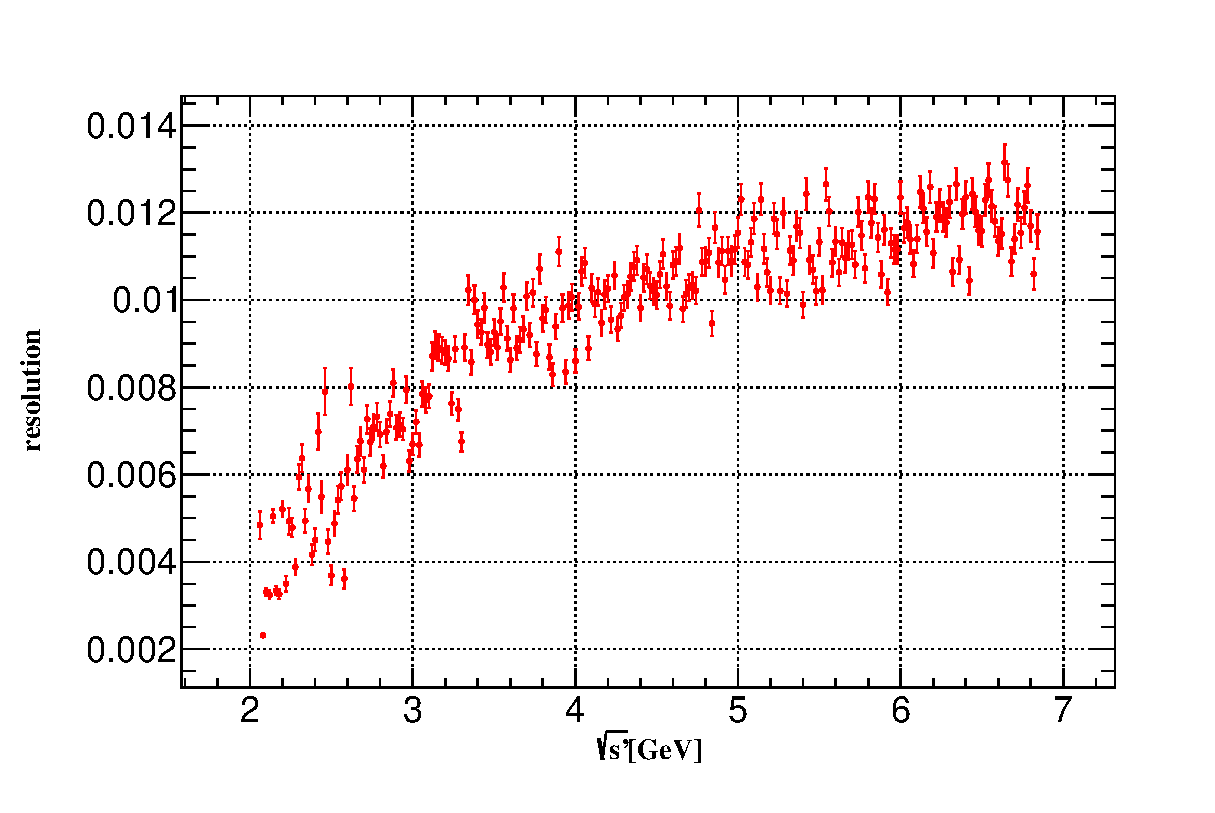
\includegraphics[width=\textwidth]{figures/divide_bin.eps}
    \end{column}

    \begin{column}{0.4\textwidth}
      \centering
      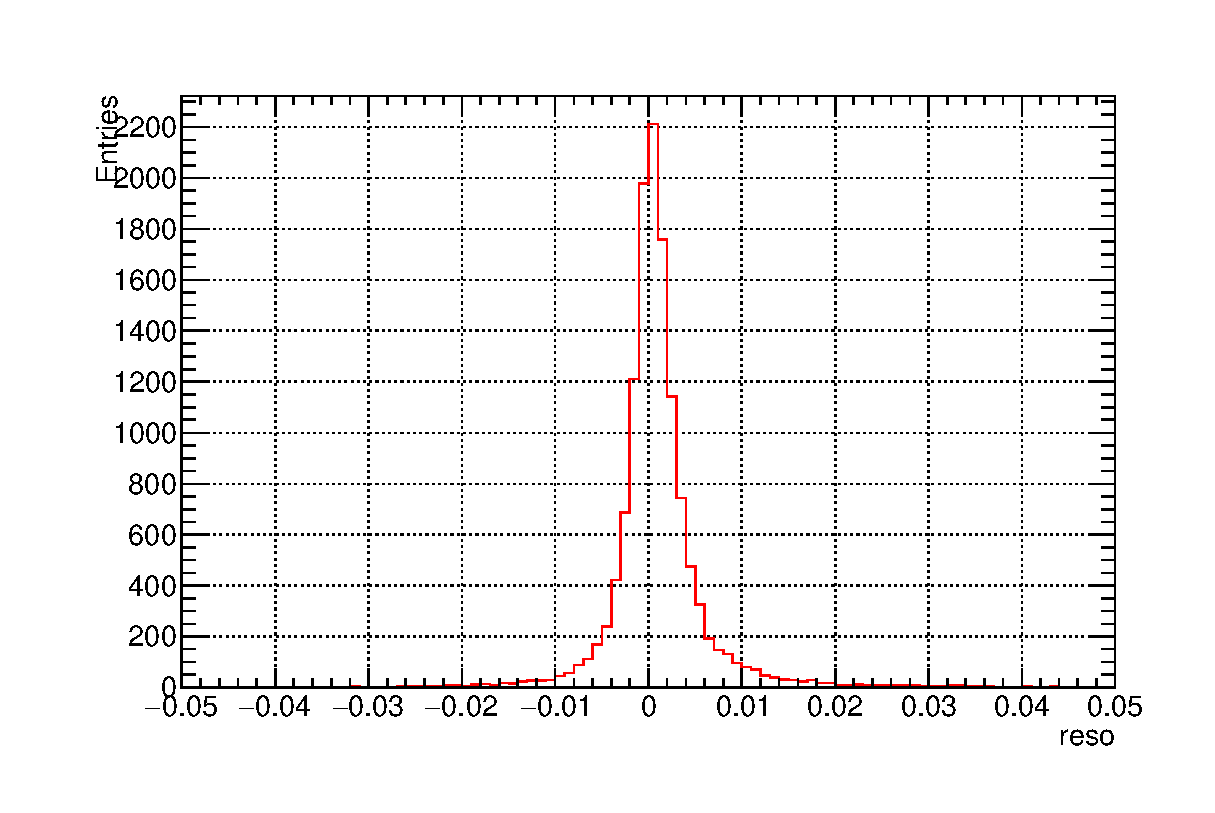
\includegraphics[width=\textwidth]{figures/reso.eps}
    \end{column}

    \begin{column}{0.33\textwidth}
      bin width:
     \begin{itemize}
      \item 25MeV at 2-3GeV
      \item 35MeV at 3-4.5GeV
      \item 40MeV at 4.5-7.5GeV
     \end{itemize}
    \end{column}
   \end{columns}
\end{frame}


\begin{frame}
  \frametitle{efficiency}
  using BW convolution a Guassian fit $\phi$ to get $N_{signal}$
 \begin{columns}
  \begin{column}{0.5\textwidth}
   \centering
   \includegraphics[width=\textwidth]{figures/sMC_phi_fit_0.png}
  \end{column}

  \begin{column}{0.5\textwidth}
   \centering
   \includegraphics[width=\textwidth]{figures/1b36c40nphi_efficiency.png}
  \end{column}
 \end{columns} 
\end{frame}


\begin{frame}
  \frametitle{Simulation vs Data}
  \begin{columns}
    \begin{column}{0.5\textwidth}
      \centering
      \includegraphics[width=\textwidth]{figures/data_vs_mc_chisq.png}
    \end{column}

    \begin{column}{0.5\textwidth}
      \centering
      \includegraphics[width=\textwidth]{figures/data_vs_mc_vpho.png}
    \end{column}
  \end{columns}
\end{frame}

\section{Branch Fraction of $J/\psi\to K^+ K^-$}


\section{Summary}


\section*{Back up}

\begin{frame}
  \begin{itemize}
    \item[$\star$] 暂时存在的一些问题:
    \begin{itemize}
    \item Data-Driving 去除本底的方式只适用于Born过程,在这里出现的主要峰状本底是$e^+e^-\to \phi \phi \gamma^I$,此方式并不合适
    \item 关于PID的优化在与又文讨论后在细节上还存有一点问题,需进一步讨论
    \end{itemize}

    \item[$\star$] to do list:
    \begin{itemize}
      \item 产生run-dependent 的signalMC ?
      \item 搞清$J/\phi$ 分支比验证的流程
      \item 其他能区的分析
    \end{itemize}


    
  \end{itemize}
\end{frame}

\end{document}
